\chapter{Z Tanım Bölgesinde Kontrolör Tasarımı}
\begin{enumerate}
    \item Geçici hal yanıtını şekillendirecek isterler dikkate alınarak s tanım bölgesinde baskın kutuplar seçilir. 
    \item Baskın kutuplar $z=e^{sT}$ ilişkisi ile z tanım bölgesine aktarılır. 
    \item Kontrol edilecek sistem Z tanım bölgesine geçirilir. 
    \item Kapalı çevrim transfer fonksiyonu elde edilir ve kutup atama yapılır.
\end{enumerate}
Örnek sistem
\begin{equation}
    G(s)=\frac{1}{s+2}
\end{equation}
z tanım bölgesinde $T=0.2$ olmak üzere
\begin{equation}
    G(z)=\frac{0.1648}{z-0.6703}
\end{equation}
olarak elde edilmektedir. Yerleşme zamanı $t_s=2$ ve aşım $\%10$ isterleri verilmiştir. Bu durumda $\zeta=0.591$ ve $w_n=6.7664$ seçilir. Seçilen sönüm oranı ve doğal frekans ile baskın kutuplar
\begin{equation}
    s_{1,2}=-4 \pm 5.4575i
\end{equation}
şeklinde hesaplanır. $z=e^{sT}$ ifadesi ile z tanım bölgesinde kutuplar
\begin{equation}
    z_{1,2}=0.2072 \pm 0.3987i
\end{equation}
ve kutuplardan oluşturulacak polinom
\begin{equation}
    p(z)=z^2-0.4144 z+0.2019
\end{equation}
olarak hesaplanır. P tipi kontrolör ile kapalı çevrim transfer fonksiyonunun ifadesi
\begin{equation}
\begin{split}
    T(z)&=\frac{kG(z)}{1+kG(z)}\\
    &=\frac{k\frac{0.1648}{z-0.6703}}{1+k\frac{0.1648}{z-0.6703}}\\
    &=\frac{k(0.1648)}{z-0.6703+k(0.1648)}\\
    &=\frac{0.1648k}{z+0.1648k-0.6703}
\end{split}
\end{equation}
şeklindedir. Görüldüğü üzere karakteristik polinom birinci dereceden elde edilmiştir ve her iki isterlerin sağlanması mümkün değildir. Yerleşme zamanı sağlanmak istenirse,
\begin{equation}
    s=-\frac{4}{t_s}=-4
\end{equation}
ve z tanım bölgesinde
\begin{equation}
    z=e^{sT}=e^{-0.8}=0.4493
\end{equation}
elde edilir. Bu durumda P kontrolör
\begin{equation}
\begin{split}
    -0.1648k+0.6703&=0.4493\\
    k&=1.341
\end{split}
\end{equation}
şeklindedir. Kapalı çevrim transfer fonksiyonu
\begin{equation}
    T(z)=\frac{0.221}{z - 0.4493}
\end{equation}
şeklindedir. Kapalı çevrim transfer fonksiyonuna ait basamak yanıtı Şekil~\ref{fig:lec6_step1} ile verilmiştir.
\begin{figure}[!htb]
    \centering
    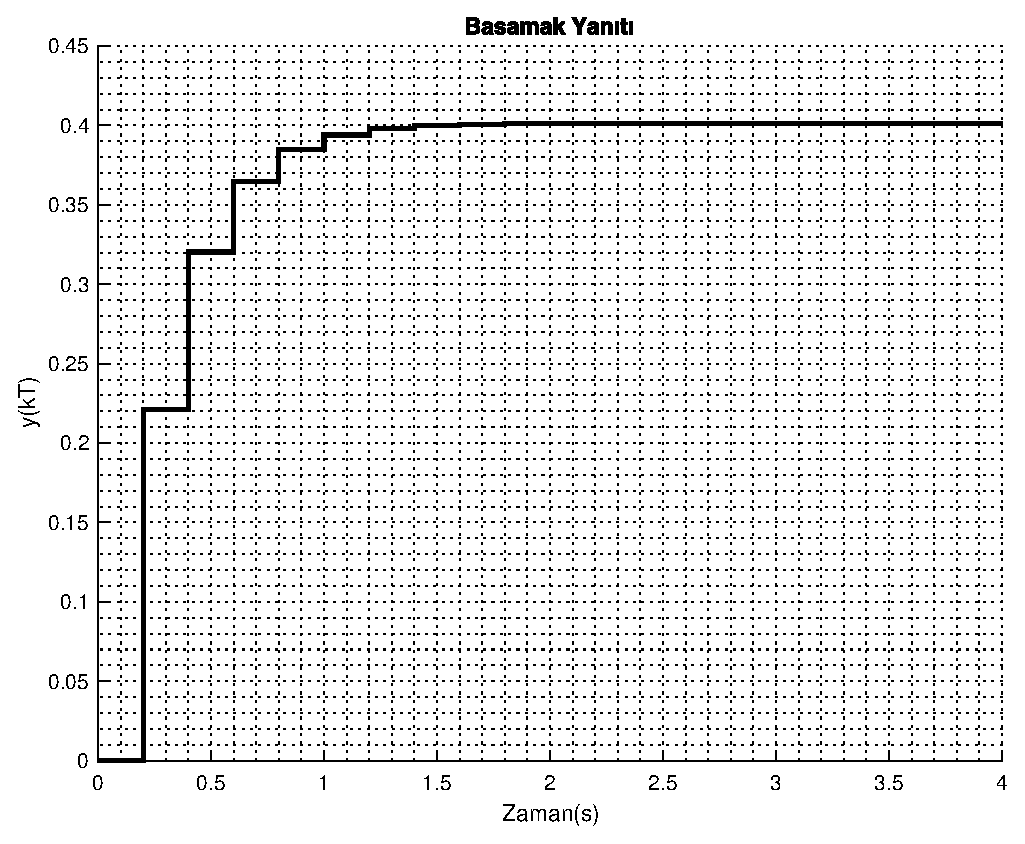
\includegraphics[width=0.75\textwidth]{img/lec6_step1}
    \caption{P kontrol için kapalı çevrim basamak yanıtı}
    \label{fig:lec6_step1}
\end{figure}

PD kontrolör transfer fonksiyonu
\begin{equation}
\begin{split}
    F(z)&=K_p+K_d(1-z^{-1})\\
    &=K_p+K_d(\frac{z-1}{z})\\
    &=\frac{K_pz+K_dz-K_d}{z}\\
    &=\frac{(K_p+K_d)z-K_d}{z}
\end{split}
\end{equation}
olmak üzere kapalı çevrim transfer fonksiyonu
\begin{equation}
    \begin{split}
        T(z)&=\frac{F(z)G(z)}{1+F(z)G(z)}\\
        &=\frac{\frac{(K_p+K_d)z-K_d}{z}\frac{0.1648}{z-0.6703}}{1+\frac{(K_p+K_d)z-K_d}{z}\frac{0.1648}{z-0.6703}}\\
        &=\frac{0.1648(K_d+K_p)z-0.1648-K_d}{z^2+(0.1648(K_p+K_d)-0.6703)z-0.1648K_d}
    \end{split}
\end{equation}
şeklindedir. Bu durumda tasarım problemi
\begin{equation}
    \begin{split}
        0.1648(K_p+K_d)-0.6703&=-0.4144\\
        -0.1648K_d&=0.2019
    \end{split}
\end{equation}
ve çözüm ise $K_d=-1.2251$ ve $K_p=2.7778$ olarak elde edilir. PD kontrolör
\begin{equation}
    F(z)=\frac{1.553 z + 1.225}{z}
\end{equation}
ve kapalı çevrim transfer fonksiyonu ifadesi
\begin{equation}
    T(z)=\frac{0.2559 z + 0.2019}{z^2 - 0.4144 z + 0.2019}
\end{equation}
olarak elde edilir.
\begin{figure}[!htb]
    \centering
    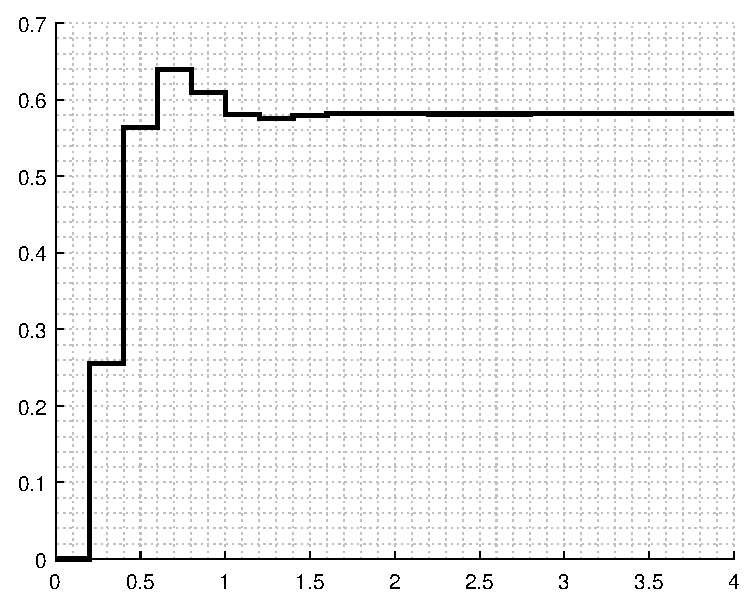
\includegraphics[width=0.75\textwidth]{img/lec6_step2}
    \caption{P kontrol için kapalı çevrim basamak yanıtı}
    \label{fig:lec6_step2}
\end{figure}

PI kontrolörü 
\begin{equation}
\begin{split}
    F(z)&=K_p+\frac{K_iz}{z-1}\\
    &=\frac{(K_p+K_i)z-K_p}{z-1}
\end{split}
\end{equation}
olarak tanımlanmıştır. Kapalı çevrim transfer fonksiyonu 
\begin{equation}
    \begin{split}
        T(z)&=\frac{F(z)G(z)}{1+F(z)G(z)}\\
        &=\frac{\frac{(K_p+K_i)z-K_p}{z-1}\frac{0.1648}{z-0.6703}}{1+\frac{(K_p+K_i)z-K_p}{z-1}\frac{0.1648}{z-0.6703}}\\
        &=\frac{0.1648(K_p+K_i)z-0.1648K_p}{z^2+(0.1648(K_p+K_i)-1.6703)z+0.6703-0.1648K_p}
    \end{split}
\end{equation}
şeklindedir. Tasarım problemi
\begin{equation}
    \begin{split}
       0.1648(K_p+K_i)-1.6703&=-0.4144\\
       0.6703-0.1648K_p&=0.2019
    \end{split}
\end{equation}
ve çözüm ise $K_p=2.8423$ ve $K_i=4.7784$ şeklindedir. Bu durumda PI kontrolör
\begin{equation}
        F(z)=\frac{7.621 z - 2.842}{z-1}
\end{equation}
ve kapalı çevrim transfer fonksiyonu
\begin{equation}
\begin{split}
    T(z)&=\frac{1.256 z - 0.4685}{z^2 - 0.4141 z + 0.2018}\\
    &=\frac{1.2562 (z-0.373)}{z^2 - 0.4141 z + 0.2018}\\
\end{split}
\end{equation}
olarak elde edilir.

\begin{figure}[!htb]
    \centering
    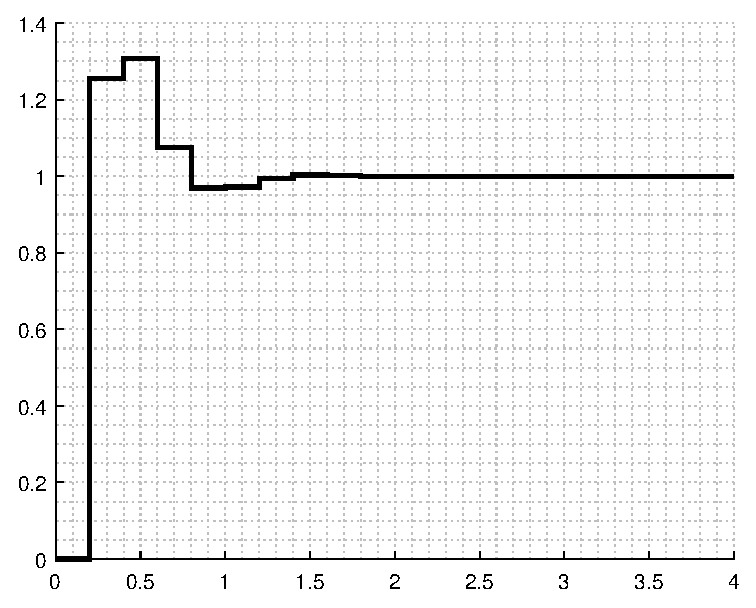
\includegraphics[width=0.75\textwidth]{img/lec6_step3}
    \caption{P kontrol için kapalı çevrim basamak yanıtı}
    \label{fig:lec6_step3}
\end{figure}